\documentclass[../thesis.tex]{subfiles}

\begin{document}
\chapter{Background}

In this chapter, we will cover the following areas: a brief history on how multi-class classification has been performed, recent approaches to the hierarchical classification problem, modern approaches to extracting useful features from images and text, and a brief overview of community detection algorithms on graphs. These areas highlight the major ideas that underpin the approaches developed in this thesis and provide context to the work that we have done.

\section{Multi-Class Classification}
When solving supervised classification tasks, the traditional assumption is that the labels, $\mathbf{y}$ in the data, $\mathcal{D} = \{(\mathbf{x}_i, y_i)\}_{i=1}^n$ are binary; that is, $y_i \in \{0, 1\}$ for $i = 1, 2, \ldots, n$. When this assumption is relaxed and $y_i \in \mathcal{L}$ where $\mathcal{L} = \{1, 2, \ldots, k\}$ for all samples, then we are dealing with a multi-class classification problem. To tackle this added complexity, past researchers have developed a number of competing approaches.

The simplest solution, as explained by Aly in a survey on multi-class classification techniques \cite{aly2005survey}, is to employ a ``one-versus-rest'' (OVR) classifier. To do this, for the $j^{th}$ class where $j \in \mathcal{L}$, all samples which correspond to label $j$ are treated as the ``positive'' class and all of the remaining classes are treated as ``negative.'' Mathematically this corresponds to re-mapping $\mathbf{y}$ such that $y_i^j = 1$ if $y_i = j$ and $y_i^j = 0$ if $y_i \neq j$ for every $i$. Using this procedure we then generate a new data set, $\mathcal{D}^\prime = \{(\mathbf{x}_i, y_i^1), (\mathbf{x}_i, y_i^2), \ldots, (\mathbf{x}_i, y_i^k)\}_{i=1}^n$. Using $\mathcal{D}^\prime$, a classifier function $f^j: \mathbf{X} \rightarrow \mathbf{y}^j$ is trained for $j = 1, 2, \ldots, k.$ To generate test set predictions, the model computes
\begin{equation}
    \label{eq:ovr_pred}
    \hat{y}_i = \underset{j \in \mathcal{L}}{\argmax} \ \  f^j(\mathbf{x}_i)
\end{equation}
where $f^j(\mathbf{x}_i) \in \R$.

In contrast with an OVR approach, an alternative methodology to solving the multi-class classification task is employ an ``all-versus-all'' (AVA) classifier. Similar an OVR classifier, AVA casts the problem as a binary classification task by re-mapping $\mathbf{y}$. However, instead of treating the $j^{th}$ label as the positive class and everything else as negative, AVA re-maps $\mathbf{y}$ by going through all $\binom{k}{2}$ label pair combinations and arbitrarily maps one as positive and the other as negative. That is, for some labels $u$ and $v$ such that $u, v \in \mathcal{L}$, $y_i^{(u,v)} = 1$ if $y_i = u$ and $y_i^{(u,v)} = 0$ if $y_i = v$. The resulting transformed data set is, $\widetilde{\mathcal{D}} = \{(\mathbf{x}_i, y_i^{(1,2)}), (\mathbf{x}_i, y_i^{(1,3)}), \ldots, (\mathbf{x}_i, y_i^{(k-1, k)})\}_{i=1}^n$. Using $\widetilde{\mathcal{D}}$, a binary classifier $f^{(u,v)}: \mathbf{X} \rightarrow \mathbf{y}^{(u,v)}$ is trained for all $(u, v) \in K$ where $K = \{(1, 2), (1, 3), \ldots, (k-1, k)\}$. To generate predictions the AVA model first computes
\begin{equation}
    \hat{y}_i^{(u,v)} = \underset{u, v}{\argmax} \ \ f^{(u,v)}(\mathbf{x}_i)
\end{equation}
for all $(u,v) \in K$ and then using the binary predictions, a final prediction is made by computing
\begin{equation}
    \hat{y}_i = \underset{j \in \mathcal{L}}{\argmax} \ \sum_{(u, j) \in K} \hat{y}_i^{(u, j)} + \sum_{(j, v) \in K} \hat{y}_i^{(j, v)}.
\end{equation}

To compare the performance of an OVR versus an AVA classifier, Hsu and Chen \cite{hsu2002comparison} trained a support vector machine (SVM) using these two training paradigms. They found that in general the AVA method outperformed OVR \textbf{WE NEED TO SCAN THE PAPER TO SUMMARIZE THE RESULTS}. However, even though AVA has demonstrated superior performance, OVR is still the preferred method. This is because OVR scales linearly in $k$ whereas AVA experiences combinatorial growth due to training $\binom{k}{2}$ classifiers.

\section{Hierarchical Classification}
In contrast with AVA and OVR classification, a third approach to the multi-class classification problem is known as hierarchical classification (we abbreviate this as HC and will interchangeably use it to mean hierarchical classification or hierarchical classifier). The main idea behind HC is that the output space, $\mathbf{y}$, is arranged into a hierarchy -- typically represented as a tree -- and this grouping is used to train a multi-class classifier. Figure \ref{fig:bin_hc} displays a simple example of an HC.

\begin{figure}
    \centering
    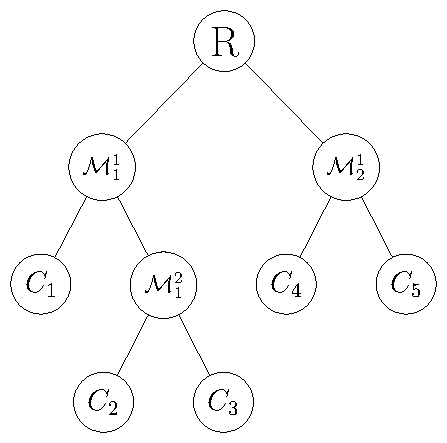
\includegraphics{images/bin_hc.pdf}
    \caption[Example Binary Hierarchical Classifier]{Example binary HC with $k = 5$ where the splits require a binary classifier as indicated since all parent nodes in the tree have a degree of two. The meta-classes, $\mathcal{M}_i^l$ correspond to the labels that have been grouped together at level $l$ and the leaves in the tree are the labels found in $\mathbf{y}$}
    \label{fig:bin_hc}
\end{figure}

To train an HC, for every node in the tree excluding the root (shown as R in Figure \ref{fig:bin_hc}), $\mathbf{y}$ is re-mapped according to the set dictated in the node. For example, in Figure \ref{fig:bin_hc}, $\mathcal{M}_1^1 = \{1, 2, 3\}$ and $\mathcal{M}_2^1 = \{4, 5\}$ so the target vector at the first level equals one if the $i^{th}$ sample belongs to $\mathcal{M}_2^1$ and equals zero if it belongs to $\mathcal{M}_1^2$. For the second level of the tree, $C_1 = \{1\}$ and $\mathcal{M}_1^2 = \{2, 3\}$ so we re-map the target using the same rule. If instead of having a purely binary HC like Figure \ref{fig:bin_hc} and instead we had a mixed tree as shown in Figure \ref{fig:ovr_hc},

\begin{figure}
    \centering
    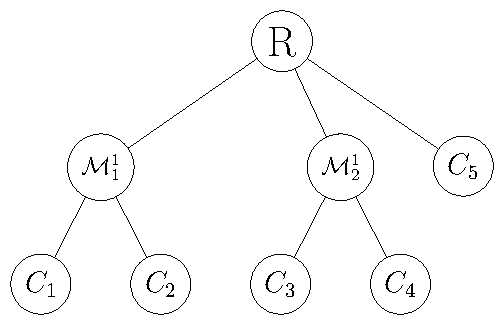
\includegraphics{images/ovr_hc.pdf}
    \caption[Example Mixed Hierarchical Classifier]{Example mixed HC for $k=5$ with the first level of the tree have an OVR classifier which predicts the labels $\mathcal{M}_1^1$, $\mathcal{M}_2^1$, and $C_5$, and the second level contains only a binary classifier.}
    \label{fig:ovr_hc}
\end{figure}

then any level where the parent node has a degree greater than two, $\mathbf{y}$ is re-mapped using the rule for an OVR classifier.

Once the data has been adjusted accordingly, then either a binary or OVR classifier is trained. To generate test sample predictions, starting at the root, the algorithm computes the label which is most likely for that level. Once this computation has been made, we move to the node which corresponds to the prediction. If the node is a leaf, then the algorithm terminates and outputs the final prediction as the label corresponding to that vertex. If the node is not a leaf, then the process is repeated until a leaf is reached.

Given the additional complexity of an HC, it is reasonable to ask why this methodology would be preferred over the simpler OVR or AVA approaches. The original reason that HC's were introduced was to decrease testing time. Some of the first authors to introduce and utilize this approach such as \cite{vural2004hierarchical}, \cite{bengio2010label}, and \cite{deng2011fast} stated that by utilizing this architecture they were able to significantly reduce the time it took to classify a particular sample. This is a useful metric to optimize when there are a large number of labels and it is important from a business perspective to make predictions as quickly as possible (such as the stock market).

To see why an HC could be faster as predicting, we will use Figure \ref{fig:bin_hc} as an example. Suppose that $y_i = 2$ and that the model is able to correctly predict this value. Using the hierarchy presented shown in Figure \ref{fig:bin_hc}, to make this classification the sample follows the path: $(R \rightarrow \mathcal{M}_1^1 \rightarrow \mathcal{M}_1^2 \rightarrow C_2$). To yield this path, the algorithm has to make three computations: predicting $\mathcal{M}_1^1$, $\mathcal{M}_1^2$, and finally $C_2$. Compare this to the OVR and AVA models. For OVR, according to (\ref{eq:ovr_pred}), the model makes five computations since there are a total of five labels in the data. An AVA model would make $\binom{5}{2} = 10$ calculations for each of the pairwise models. What this demonstrates, is that an HC has the potential, with the correct hierarchy, to significantly reduce the time to takes to classify a sample. 

Having introduced the two most common approaches to mutli-class classification and HC, we will now dive more deeply into the necessary components of an HC and previous approaches to provide context to how we are solving the problem. First we will start with the problem of inferring a hierarchy from data.

\section{Hierarchy Inference}
To utilize an HC, the grouping must either be known a-prior or it must be inferred from the data. As Silla and Freitas describe in \cite{silla2011survey}, there is a significant body of work when the hierarchy is known beforehand. However, an open problem is how find the best label grouping when it is not known. In some ways, this challenge can be viewed as an unsupervised learning task and hence there are a number of competing, and sensible approaches, to this problem.

One of the first attempts proposals to solving the hierarchy inference (HI) problem was proposed by Vural and Dy in \cite{vural2004hierarchical}. In their paper, they introduce the ``Divide-by-2'' (DB2) method. What they propose to is formulate a binary decision tree, like Figure \ref{fig:bin_hc}. The key challenge in this problem is how best to go about building this tree. To solve this challenge, the authors introduce three different heuristics.

The first one is what they call: ``K-means Based Division.'' To implement this algorithm, they represent each label in the data using a single point $\mathbf{v}_j$ where $\mathbf{v}_j$ equals
\begin{equation}
    \mathbf{v}_j = \frac{1}{m_j} \sum_{\mathbf{x}_i \in C_j} \mathbf{x}_i
\end{equation}
where $m_j$ is the number of samples in class $C_j$. Using $\mathbf{v}_j$, Vural and Dy then propose to solve the k-means clustering problem:
\begin{equation}
    \label{eq:k_means}
    \underset{S}{\argmin} \ \ \sum_{i=1}^2 \sum_{\mathbf{v} \in S_i} \left \Vert \mathbf{v} - \boldsymbol{\mu}_i \right \Vert_2^2
\end{equation}
where the number of clusters, $k$ is set to two. If $S_i$ for $i = 1, 2$ is a singleton, that is there is only one label in the cluster, then we stop; otherwise, the labels in $S_i$ are clustered again using (\ref{eq:k_means}). This process is applied recursively until every cluster has a single label in it. For example, in Figure \ref{fig:bin_hc}, applying k-means based division the first time yielded the clusters $\mathcal{M}_1^1 = \{1, 2, 3\}$ and $\mathcal{M}_2^1 = \{4, 5\}$. Applying the (\ref{eq:k_means}) again to the labels in $\mathcal{M}_1^1$ we get $C_1 = \{1\}$ and $\mathcal{M}_1^2 = \{2, 3\}$. Since $C_1$ is a singleton, the algorithm stops, but $\mathcal{M}_1^2$ has more than one element so we call it again. Since both $\mathcal{M}_1^2$ and $\mathcal{M}_2^1$ have a cardinality of two, their final clusters would be singletons. Since all clusters now contain a single label, the terminating condition has been met. Although Vural and Dy propose this k-means based heuristic, in their paper, they do not provide any experimental results for the method. Instead they just decided to provide results for the case where they create balanced subsets of the labels. Additionally, to the best of my our knowledge, no other paper which used HC as the primary classification methodology has utilized the k-means based inference approach. 

In our work, we use this k-means clustering idea in two ways. The first, is that we directly use the heuristic, but instead of requiring that $k=2$ we treat the number of cluster or meta-classes as a hyper-parameter which needs to be inferred via cross-validation. We are able to take this approach because our objective, unlike the original authors, is not to create a generic binary classifier, but rather to produce a classifier which is able to perform well when there are a large number of similar labels. The second way in which we use this k-means clustering idea is by formulating the problem as a mixed-integer program. We will provide more details in Chapter 3. 

The second technique that Vural and Dy introduce is what they call the ``Spherical Shells'' method. They implement this algorithm using $\mathbf{v}_j$ and the grand mean $\mathbf{m}$ computed as
\begin{equation}
    \mathbf{m} = \frac{1}{n}\sum_{i=1}^n \mathbf{x}_i.
\end{equation}
With $\mathbf{m}$ as a threshold, if $\left \Vert \mathbf{v}_j \right \Vert_2 \leq \left \Vert \mathbf{m} \right \Vert_2$ then label $j$ is mapped to the negative class; otherwise, it is the positive class. This rule is again applied recursively until the leaves of the tree contain only one label and where the grand mean is updated to reflect the composition of the vertex. For example, if we used this rule and got Figure \ref{fig:bin_hc} as the inferred hierarchy, then then $L_2$ norm of labels one, two, and three were less than or equal to the grand mean of the root, $\mathbf{m}^R$. To compute the split for the vertex $\mathcal{M}_1^1$, the grand mean is $\mathbf{m}^{\mathcal{M}_1^1}$ and the $L_2$ norm of $\mathbf{v}_1$ is less than or equal to $\mathbf{m}^{\mathcal{M}_1^1}$ and $\mathbf{v}_2$ and $\mathbf{v}_3$ are greater than the grand mean. The algorithm recurses until all of the leaves are single classes.

The final technique that Vural and Dy detail is what they call ``Balanced Subsets.'' With this heuristic, the authors generate the label hierarchy by,  ``...dividing the data into two subsets such that difference in the number of samples in each subset is minimum.'' They state that this is a useful heuristic if the speed of the process is important or if there is a skewed label distribution.  Moreover, as mentioned earlier, this is the technique that the authors used for their experiments in their paper, and in their work, they demonstrate that by employing their ``DB2'' model, that they are able to achieve comparable performance relative to other multi-class classifiers such as OVR or AVA approaches while significantly decreasing the time it takes to classify a test sample. In this work, however, the test set prediction time is not something that we are care about; rather, we are mostly concerned with improving the performance of the estimator in the presence of a large number of labels.

The second major attempt at hierarchical classification, which proposed a technique seems quite popular today was created by Bengio, Weston, and Grangier in their work, \textit{Label Embedding Trees for Large Multi-Class Tasks} \cite{bengio2010label}. The goal of this work was similar to that of Vural and Dy's -- the authors wanted to implement a mutli-class classifier which was able to compute test set predictions more quickly than the standard OVR or AVA approach. However, unlike \cite{vural2004hierarchical}, Bengio, Weston, and Grangier inferred the label hierarchy by tying it to the performance of an classifier rather than using a clustering heuristic. In particular, they propose the following simple algorithm to infer the label hierarchy and train the corresponding HC:

\begin{algorithm}[H]
    \caption{Spectral Clustering HC}
    \label{alg:bengio_approach}
    \begin{algorithmic}[1]
        \Procedure{trainSpectralHC}{$\mathbf{X}$, $\mathbf{y}$, $k$}
            \State Train a OVR classifier using $\mathbf{X}$ and $\mathbf{y}$
            \State Compute the confusion matrix $\mathbf{C}$ on the validation set, $\mathcal{V}$
            \State Get the affinity matrix $\mathbf{A} = \frac{1}{2}\left(\mathbf{C} + \mathbf{C}^T\right)$
            \State $\mathbf{Z}_{SC} \gets $ Perform spectral clustering on $\mathbf{A}$ with $k$ clusters
            \State Train a HC using $\mathbf{Z}_{SC}$ as the label hierarchy
        \EndProcedure
    \end{algorithmic}
\end{algorithm}

Before explaining the intuition behind Algorithm \ref{alg:bengio_approach}, I first need to briefly explain spectral clustering. Spectral clustering is a popular unsupervised learning algorithm that attempts to partition the provided data points by transforming the data matrix, $\mathbf{X}$ into a new space then using a simple clustering algorithm, like k-means clustering, to group them. In their paper, \textit{On Spectral Clustering: Analysis and an algorithm} \cite{ng2002spectral}, Ng, Jordan, and Weiss, propose a simple algorithm that is commonly implemented in a number of open-source machine learning packages, like Python's scikit-learn, to solve the spectral clustering problem. Specifically they do the following steps:
\begin{enumerate}
    \item Form an affinity matrix, $\mathbf{A} \in R^{n \times n}$ by computing the radial basis function (RBF) kernel. The RBF kernel is defined as
    \begin{equation}
        K(\mathbf{x}, \mathbf{y}) = \exp\left(-\frac{\lVert \mathbf{x} - \mathbf{y}\rVert_2^2}{2\sigma^2}\right)
    \end{equation}
    \item Compute the Laplacian, $\mathbf{L}$, by calculating $\mathbf{L} = \mathbf{D}^{-1/2}\mathbf{A}\mathbf{D}^{-1/2}$ where $\mathbf{D}$ is a diagonal matrix whose $(i, i)$-element is the sum of $\mathbf{A}$'s $i^{th}$ row
    \item Compute the $k$ largest eigenvectors, $\mathbf{x}_1, \mathbf{x}_2, \ldots, \mathbf{x}_k$ from $\mathbf{L}$ and form a new matrix, $\mathbf{Y} = [\mathbf{x}_1 \mathbf{x}_2 \cdots \mathbf{x}_k] \in \R^{n \times k}$ by stacking the eigenvectors in a column. 
    \item Finally normalize $\mathbf{Y}$ and perform k-means clustering on the matrix to generate the partition of the samples. 
\end{enumerate}
At a high level, by transforming the data matrix, $\mathbf{X}$ from its normal features space into a new one based off its eigenvectors this will separate the data points and make it easier to cluster. 

Returning to inferring a label hierarchy by using spectral clustering, the intuition behind this approach is that the resulting affinity matrix $\mathbf{A}$ described in Algorithm \ref{alg:bengio_approach} will be sparse. Specifically for a given label $j$, if the original multi-class classifier is trained well, then the estimator should not be confuse class $j$ for a large number of other categories; it is likely that it is a small subset of the labels which causes the confusion. Consequently, by then performing spectral clustering on $\mathbf{A}$, these labels groups can then be teased out and a classifier which focuses on just those classes can then be trained. This idea, due to its simplicity and also theoretical soundness, has been employed in a wide range of other hierarchical classification settings. For example, in their work, \textit{HD-CNN: Hierarchical Deep Convolutional Neural Networks for Large Scale Visual Recognition} \cite{yan2015hd}, Yan et. al. implement a hierarchical convolutional neural network (CNN) by employing a similar idea that Bengio proposes. Namely, they first train a CNN which can predict all of the labels, they then use this classifier to compute a confusion matrix and perform spectral clustering on the matrix to get the label hierarchy, and finally the authors train the full HC composed only of CNNs by using this label hierarchy. This idea is also employed by Wang et. al. in their work \textit{Learning Fine-grained Features via a CNN Tree for Large-scale Classification} \cite{wang2018learning}. The idea is quite similar: train a classifier, use the performance of the initial estimator to infer the label groups, and then finally train the full HC. Instead of using spectral clustering, the authors use a heuristic inspired from integer programming, but the idea remains the same -- tie the existence of metaclasses to the performance of the initial classifier. 

In our work, we benchmark the approaches that we will introduce in Chapter 3 against the general algorithm that Bengio proposes in his work. Additionally, we also take the approach detailed in Algorithm \ref{alg:bengio_approach} and generalize it beyond the case of a OVR classifier.

Having detailed the relevant methods needed to understand multi-class and hierarchical classification, we will now discuss relevant methods for transforming our data which we use extensively for our computational experiments, and also provide some additional mathematical background for the methods that we introduce in Chapter 3.

\section{Image Feature Extraction}
A number of the data sets which we use to evaluate the performance of various classifiers contain images. Images are difficult to work with because they can contain a large number of features. For example, suppose the data contains an image which is $(256 \times 256 \times 3)$ where the $256$ indicates the number of pixels and three denotes that there are three color channels -- red, green, and blue. If one were to flatten image from a three-dimensional tensor into a vector which could be used by standard machine learning algorithms, this would yield a vector, $\mathbf{x} \in \R^{196,608}$! This is extremely high-dimensional and would be computationally intractable for most, if not all common machine learning algorithms. Additionally, images have a number of complexities that are not present with standard data sets. For example, neighboring pixels tend to be highly correlated with one another and the location of objects in images is meaningful. Consequently, simply flattening in am image tensor is not an appropriate technique because it would corrupt this necessary context for understanding what is contained in a picture. 

To deal with these issues, researchers in image processing in previous decades have developed a number of techniques which attempt to capture a low-dimensional representation of the image while respecting the complexities of working in a visual domain.

\subsection{Early Efforts}
The simplest of these approaches were edge detectors, such as the Sobel operator or Robert's Cross operator \cite{sobel19683x3} and \cite{roberts1963machine}. In both of these papers the authors introduce filters -- a $3 \times 3$ for Sobel and $2 \times 2$ for Roberts -- where the objective is to perform a convolution operation over the desired image. Ideally, if the computation yields a large value then this indicates that there is likely an edge present in that portion of the image. Figure \ref{fig:sobel_filter} displays the most common representation of a Sobel filter.

\begin{figure}
    \centering
    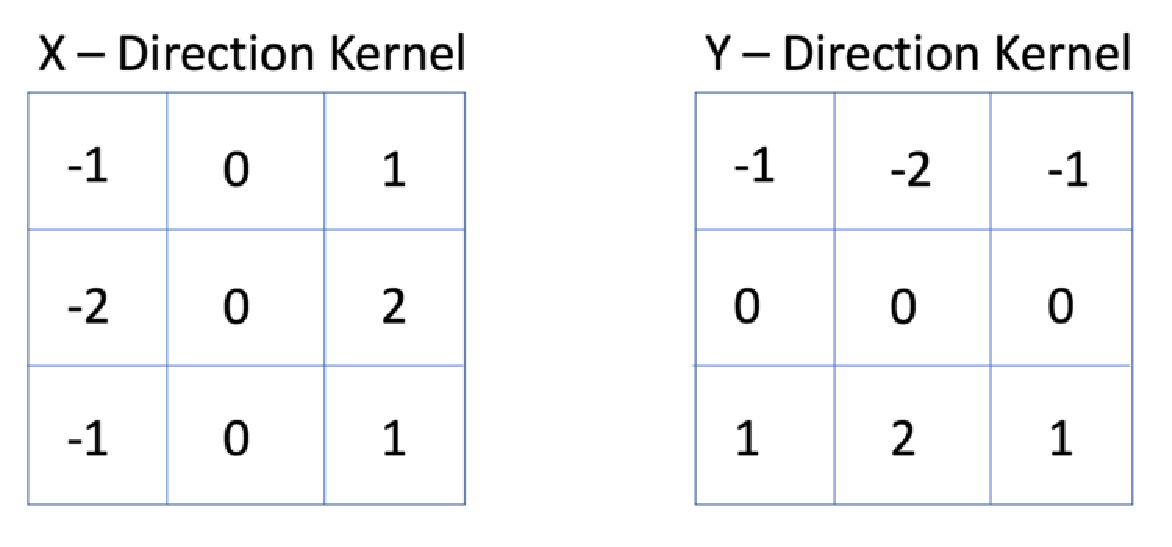
\includegraphics[width=.7\linewidth]{images/sobmasks.pdf}
    \caption[Sobel Filter]{The $x$ and $y$ filters represent the most common Sobel filters. They are designed to detect edges at $90$ degrees. There are generalizations for rotations of images.}
    \label{fig:sobel_filter}
\end{figure}

While filters such as the Sobel filter and others have enjoyed great amount of practical use for image feature extraction, their primary limitation is that they must be hand-crafted. This necessarily makes it difficult to capture more complex things in an image -- such as the presence of a face in a picture. A human face has a number of complexities to it: curves around the eyes, eyebrows, chin shape, and many others. Designing a filter or even a series of filters which could robustly identify a wide range of human faces would be extraordinarily challenging. Therefore, one of the major focuses of computer vision researchers in the early 2000s was to develop new algorithms to extract features from images that were robust to things like rotation and scale of the image.

One of the first major algorithms that was designed to be more robust than your standard filter, especially when it came to the scale of objects in images being different was a technique developed called Scale-Invariant Feature Transform (SIFT) by Lowe in 2004 in his paper, \textit{Distinctive Image Features from Scale-Invariant Keypoints} \cite{lowe2004distinctive}. In his approach, Lowe proposes to find ``keypoints'' such as edges and corners and to do so in a way that was independent of the scaling of the image. He did this by using existing corner and edge detectors and applying a threshold heuristic to account for the issue of scaling. Another work that built off the work of Lowe's SIFT was the algorithm proposed by Bay et. al. in their work, \textit{SURF: Speeded Up Robust Features} \cite{bay2006surf}. The authors propose a similar approach to SIFT, but do so in a way that dramatically decreases computation time. There are a large number of filter-based feature extraction technique which varying degrees of human intervention in their creation. In general though, one of the primary ways of extracting features from images, prior to convolutional neural networks (CNNs) was to either build or utilize an existing set of filters and apply them to detect edges, corners, or other likely points of interest in the picture.

\subsection{Convolutional Neural Networks}
However, in the past decade, the primary approach of extracting features from images using hand-crafted filters such as SIFT and SURF has shifted to a new paradigm where filters are inferred from the data, typically by employing an algorithm known as a convolutional neural network. The core idea of CNNs is that instead of relying on humans designing filters, where it is difficult to account for the wide variety of objects that could reasonably occur in an image, instead we should find filters which are optimal for the particular data set by using classification error as the mechanism for determining a ``good'' or ``bad'' set of filters. To give context on how CNNs have become more popular for feature extraction in recent years, the first major usage of CNNs was proposed by Yann LeCun in his paper, \textit{Object Recognition with Gradient-Based Learning} \cite{lecun1999object}. In this work LeCun utilizes CNNs to solve a problem of identifying hand-written digits (this a data is known as MNIST and it is commonly used a benchmark for image recognition algorithms). However, even though though CNNs showed great promise, they received little research attention (primarily due to the necessity of having large quantities of data and enormous computational resources) until they were utilized in the ``ImageNet'' challenge \cite{russakovsky2015imagenet}. This is another benchmark data set used to evaluate the performance of image detection algorithms. When the competition was initially started in 2010, the best competitor has an error rate of approximately $33.6\%$; however, in 2012, using a CNN now known as ``AlexNet,'' Krizhevsky and his co-authors were able to halve this error rate to around $16.4\%$ \cite{krizhevsky2012imagenet}. This use of a CNN has led to a flurry of other developments in the field. We will not rehash every major step forward with CNNs, but rather we will focus on how they primarily used in the context of our problem space: as feature extractors via ``transfer learning.'' 

Transfer learning is the idea that filters which are inferred by CNNs from one task (e.g, ImageNet) can be applied to other visual problems. One of the first times this technique was employed was by Razavian et. al. in their paper, \textit{CNN Features off-the-shelf: an Astounding Baseline for Recognition} \cite{sharif2014cnn}. In their work, they utilized an existing CNN model and used its features to perform image classification in a variety of different domains from the original model such as scene classification and sculpture image retrieval. This process of extracting features is nicely summarized by Figure \ref{fig:transfer_learning}. At a high level, transfer learning proposes to use features that were inferred from the original CNN and apply it to a new domain. The ``learned weights'' shown in the bottom half of Figure \ref{fig:transfer_learning}, while displayed as a neural network, can be viewed more generally as a classifier with parameters to infer for some new classification task. Moreover, the ``pre-trained weights'' can be seen as a feature extractor which transforms the input image into some new vector, $\mathbf{x} \in \R^p$. By using the pre-trained CNN and extracting its features, Razavian et. al. were able to achieve excellent performance at low computational cost because the authors were simply training a support vector machine on the extracted features. 

The transfer learning concept is used heavily throughout our image-based experiments for the same reason that \cite{sharif2014cnn} used it -- it tends to yield powerful features at low computational cost. While there are a large number of CNNs available with pre-trained weights, we specifically chose the NASNet \cite{zoph2018learning}. This was a CNN designed by $2018$ and we selected it because this model is currently the best performing on the ImageNet benchmark, and its weights are also freely available via the Keras application programming interface (API) -- a common tool used for designing neural networks in the Python programming language \cite{chollet2015keras}.

\begin{figure}
    \centering
    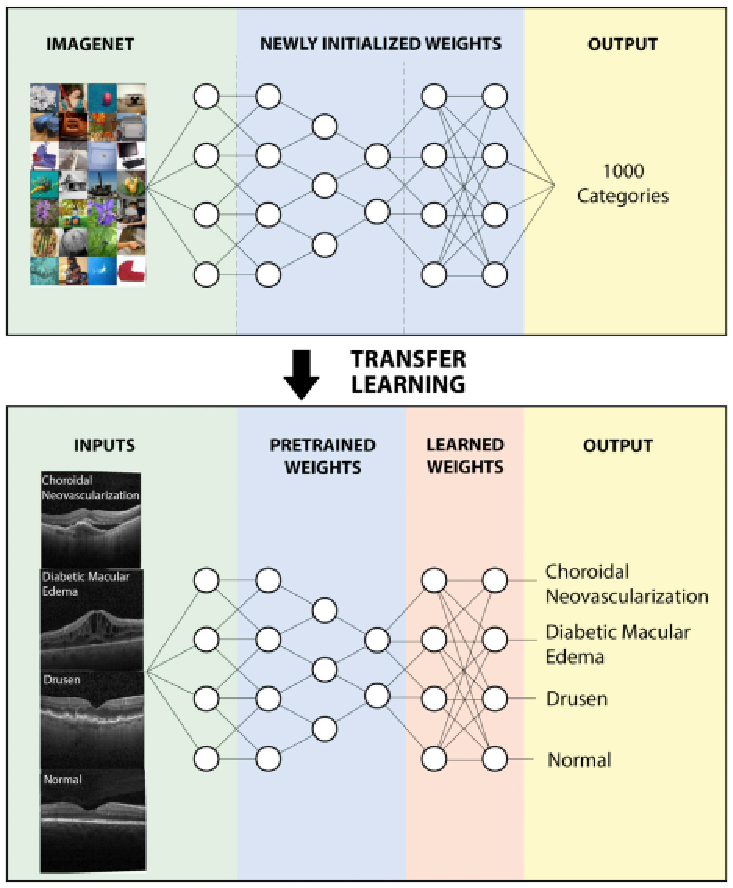
\includegraphics[width=\linewidth]{images/transfer_learning.pdf}
    \caption[Transfer Learning Example]{This displays transfer learning in the context of using a pre-trained model on the ImageNet data set, and then applying it to a new medical domain. The figure implies that one would use a neural network as the final classifier, but this notion can be generalized to almost any classifier.}
    \label{fig:transfer_learning}
\end{figure}

\section{Text Feature Extraction}
Another common technique that we will employ for the natural language processing (NLP) experiments is a concept known as ``word embeddings.'' One of the major challenges with NLP tasks is to convert a phrase such as
\begin{quote}
    The quick brown fox jumped over the lazy brown dog
\end{quote}
into something that a machine learning model can work with to make predictions, especially for our case of document classification.

\subsection{Early Approaches}
One common technique is employ an algorithm known as ``Term Frequency-Inverse Document Frequency'' (TF-IDF) \cite{sparck1972statistical}. What TF-IDF does is first count the frequency of words in a given document (term frequency) and then compute the logarithm of the reciprocal of its frequency in the entire corpus (inverse document frequency). This algorithm was first proposed in 1972 by Karen Sparck Jones and has often been paired with a Naive Bayes Classifier -- a machine learning algorithm which assumes that all features are conditionally independent of one another -- to perform tasks such as document classification \cite{kibriya2004multinomial}. However, while TF-IDF is a simple but powerful technique, it has a few primary shortcomings:
\begin{enumerate}
    \item It computes document similarity directly in the word-count space, which may be slow for large vocabularies.
    \item It assumes that the counts of different words provide independent evidence of similarity.
    \item It makes no use of semantic similarities between words \cite{tfidf_lecture}.
\end{enumerate}
To overcome these pitfalls, one of the most popular techniques has been embed words as vectors in a low dimensional space -- commonly referred as ``word embeddings.''

\subsection{Word Embeddings}
One of the most recent innovations in NLP is that words can be represented as vectors in a low-dimensional space (relative to the size of the vocabulary) and that these representations can be meaningfully used to perform useful NLP-related tasks. One of the first major implementations of this methodology was in 2013 by Mikolov et. al in the paper, \textit{Distributed Representations of Words and Phrases
and their Compositionality} \cite{mikolov2013distributed}. In this work, the authors propose to represent words as vectors (typically shortened as Word2Vec) by implementing a ``negative sampling objective.'' A negative sampling objective is defined as
\begin{equation}
    \log \sigma\left(v_{\text{WO}}^\prime \cdot v_{\text{WI}}\right) + \sum_{i=1}^k \mathbb{E}_{w_i \sim P_n(w)} \left[\log \sigma(-v_{\text{WI}}^\prime \cdot v_{\text{WI}}\right].
\end{equation}
The authors state that this objective proposes to distinguish the target word, $w_O$ by using noisy draws from the distribution $P_n(w)$. Using this algorithm, the authors were able to demonstrate that their inferred word embeddings discovered semantically meaningful relationships. For example, one of the most commonly used pictures describing this relationship is displayed in Figure \ref{fig:word2vec}.

\begin{figure}
    \centering
    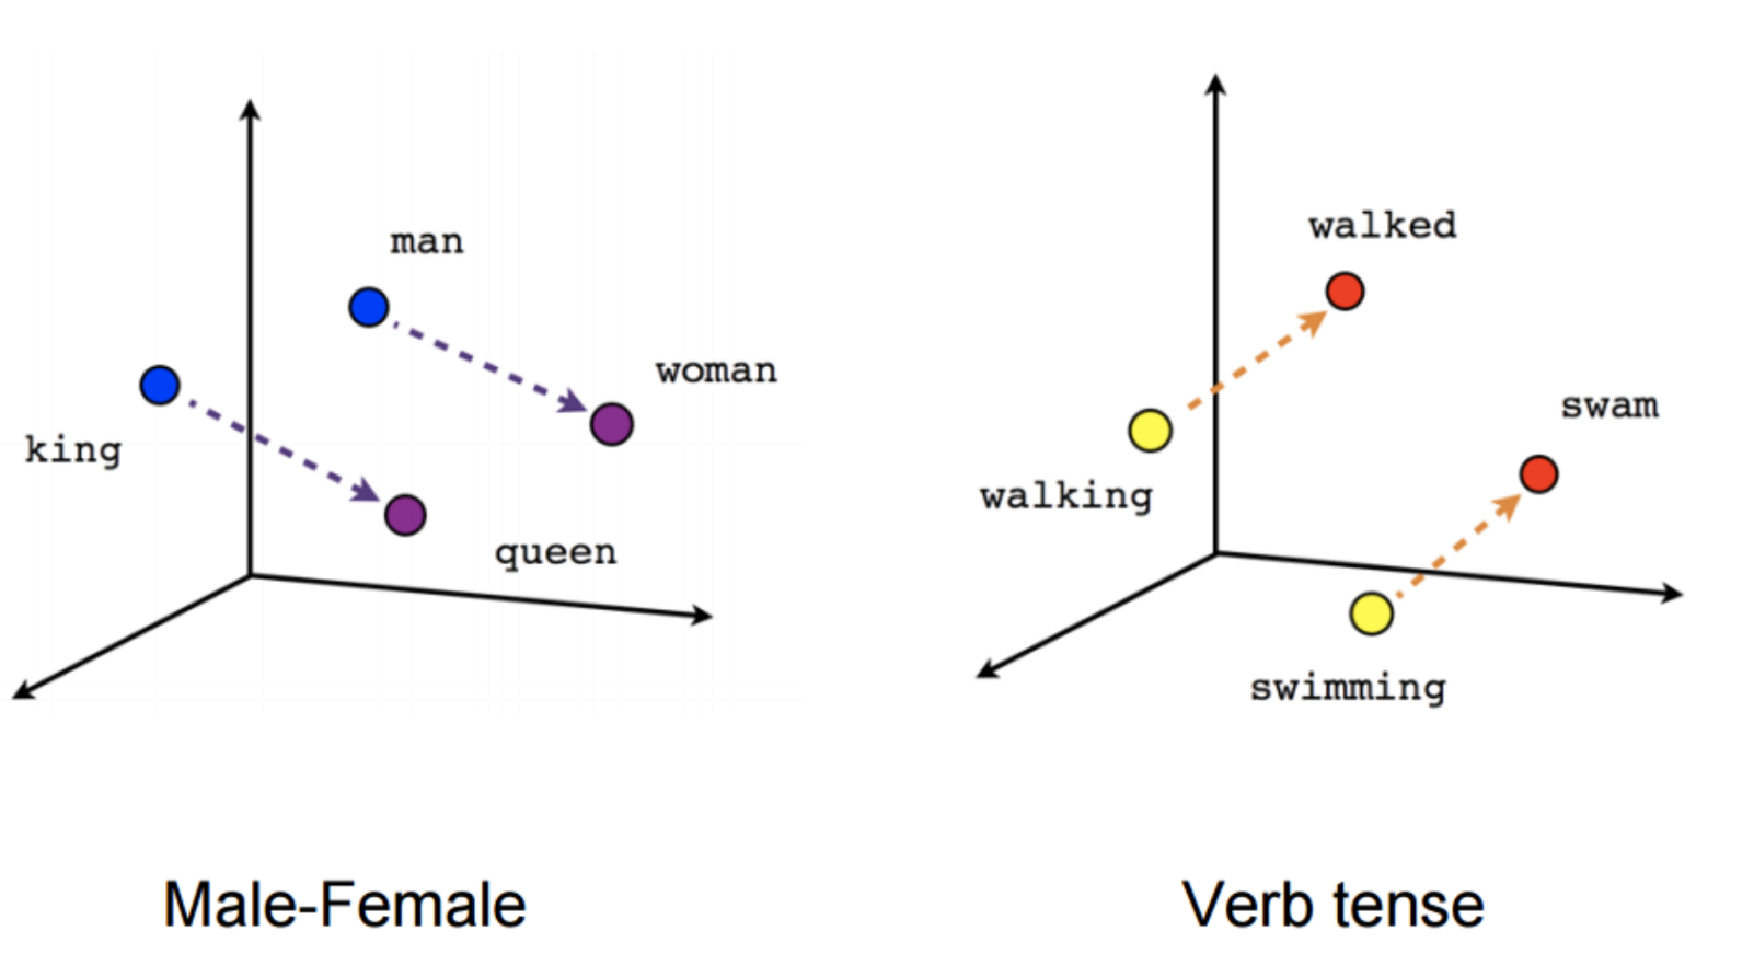
\includegraphics[width=\linewidth]{images/word2vec.pdf}
    \caption[Word2Vec Example]{To build this image, the authors of \cite{mikolov2013distributed} represented their embedded vectors in two dimensions using principal component analysis.}
    \label{fig:word2vec}
\end{figure}
Figure \ref{fig:word2vec} demonstrates that by representing words as low-dimensional vectors they were able to capture semantically meaningful relationships without using a supervised objective or providing hand-crafted rules. For example, the authors discovered that if they computed:
\begin{equation*}
    \mathbf{v}_{\text{Berlin}} - \mathbf{v}_{\text{Germany}} + \mathbf{v}_{\text{France}}
\end{equation*}
that this computation yielded the vector for Paris. This small example demonstrated that their approach can represent complex, higher-order relationships and then capture them using simple mathematical operations such as addition and subtraction. 

Building off of Mikolov's work, more recent works have used this idea of representing words as low-dimensional emebddings. One of the most popular representations, and the one that we use for the numerical experiments with text data, is ``Global Vectors for Word Representation'' (GLoVe) \cite{pennington2014glove}. To represent words as vectors, Pennington et. al. first build the matrix, $\mathbf{X}$ which is defined as the ``co-occurence'' matrix where $x_{ij}$ indicates the number of times word $j$ occurs in the context of word $i$. They they define $\mathbf{X}_i = \sum_k X_{ik}$ to be the number of times any word appears in the context of word $i$. To infer vectors which represent words, the authors propose to solve the following least squares problem
\begin{equation}
    \label{eq:glove}
    J = \sum_{i, j}^V f(x_{ij})\left(\mathbf{w}_i^T \tilde{\mathbf{w}}_j + b_i + \tilde{b}_j - \log\left(x_{ij}\right) \right)^2
\end{equation}
where $\mathbf{w}_i$ and $b_i$ defines the word vector and bias term, respectively for the $i^{th}$ word, $f(x_{ij}$ is a weighting function, and $V$ is the size of the vocabulary. To select the function, $f$, the authors stated that it should satisfy the following three properties:
\begin{enumerate}
    \item $f(0) = 0$
    \item $f(x)$ is non-decreasing
    \item $f(x)$ should be small for large values of $x$
\end{enumerate}
Using those requirements as a starting point, the Pennington found that
\begin{equation}
    \label{eq:glove_function}
    f(x) = 
    \begin{cases}
        \left(\frac{x}{x_{\text{max}}}\right)^\alpha, &\text{if } x < x_{\text{max}} \\
        1, &\text{ otherwise}
    \end{cases}
\end{equation}
worked well when they set $\alpha = \frac{3}{4}$. To optimize over (\ref{eq:glove}), the authors leveraged matrix factorization techniques and local context window methods. Their analysis demonstrates that this method of generating word embeddings gave state of the art results in $2015$. 

In our work, we utilize the GloVe vectors for two reasons: one, they are freely available on spaCy -- a NLP API available in the Python programming language -- and two, because a standard technique for document classification is to use word embeddings combined with a continuous bag of words (CBOW) model to represent documents and then feed that into a machine learning model to make predictions \cite{mikolov2013efficient}.

\section{Community Detection}
One of the techniques which we propose for inferring the label groups of a data employs community detection on graphs. Therefore to provide context on the methods we will briefly discuss some of the key ideas behind the community detection algorithms we are using.

To start, we need to provide some basic definitions of what \textit{is} a graph. Graphs (also referred to as networks) are defined by the tuple, $\mathcal{G} = (\mathcal{V}, \mathcal{E})$ where $\mathcal{V}$ is the set of vertices or nodes, and $\mathcal{E}$ is the set of edges or links. An edge connects nodes to one another. An example of a graph is displayed in Figure \ref{fig:simple_graph}.

\begin{figure}
    \centering
    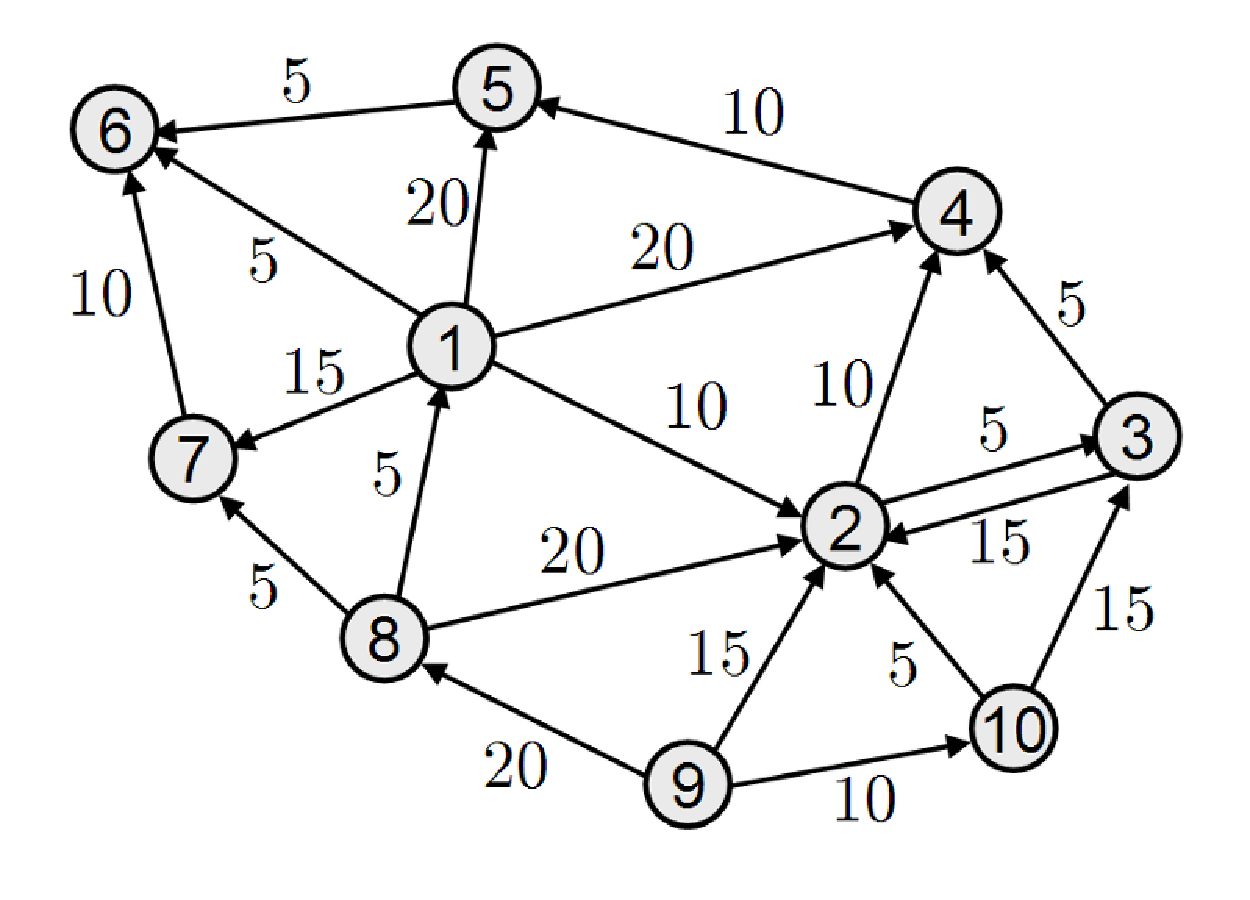
\includegraphics[width=.7\linewidth]{images/simple_graph.pdf}
    \caption[Example Graph]{This an example of a weighted, directed graph. The weights the edge, in this context, denote information flow between the vertices}
    \label{fig:simple_graph}
\end{figure}
In Figure \ref{fig:simple_graph}, the vertices, $\mathcal{V} = \{1, \ldots, 10\}$, and one element from the edges set, $\mathcal{E}$ is $(1, 5)$ where the first index denotes the starting node and the second index indicates the terminating node. 

Networks, can occur in a wide variety of contexts. For example, they have been employed on social network analysis \cite{wasserman1994social}, understanding pandemics \cite{gomez2017network}, and Google's algorithm, ``PageRank'' on their search engine \cite{page1999pagerank}. Additionally, a large number of networks display a community structure -- i.e., the vertices are organized into a group -- commonly referred to as ``communities'' or ``clusters.'' \cite{fortunato2016community}. For example, in Figure \ref{fig:simple_cd}, there are clearly three communities present in the network. One way to detect that these communities are present is through that fact that within the community there is large number of edges between the vertices, but outside of the community the number of connections is low. This idea is essential to a number of community detection algorithms and also underpins the approach that we use in our problem: modularity maximization.

\begin{figure}
    \centering
    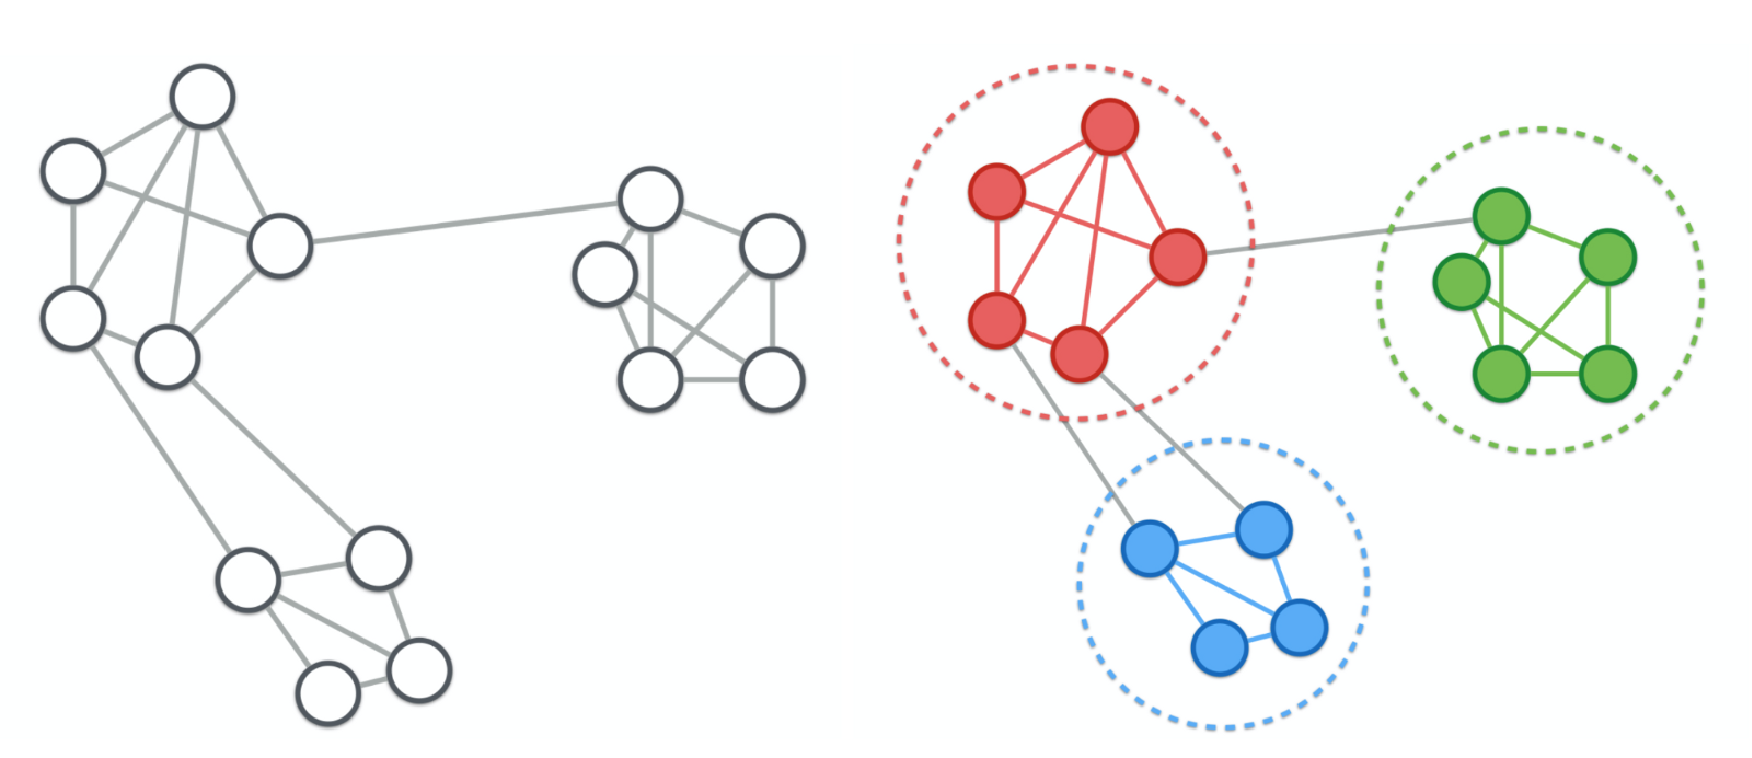
\includegraphics[width=.7\linewidth]{images/comm_detection.pdf}
    \caption[Simple Community Detection Example]{A simple example of a graph with three communities}
    \label{fig:simple_cd}
\end{figure}

\subsection{Modularity Maximization}
One of the most popular ways to infer communities is network is find a partition which maximizes the ``modularity'' of a particular graph. This technique was first introduced by Gavin and Newman in their paper, \textit{Finding and evaluating community structure in networks} \cite{newman2004finding}, where they attempt to optimize the modularity function which is defined as
\begin{equation}
    Q = \frac{1}{2m} \sum_{i,j} \left(A_{ij} - \frac{k_i k_j}{2m} \right)\mathbbm{1}(c_i = c_j)
\end{equation}
where $k_i$ and $k_j$ are the sum of the weights attached to nodes $i$ and $j$, respectively, $2m$ is the sum of all of the edge weights in the graph, $A_{ij}$ is the value of the affinity matrix at entry $(i, j)$ -- this a conversion of the tuple $\mathcal{G} = (\mathcal{V}, \mathcal{E})$ into a matrix to make it easier to perform computations -- and $c_i$ and $c_j$ are the inferred communities for nodes $i$ and $j$. Intuitively, modularity attempts to measure the difference between the realized weight between nodes $i$ and $j$ and the probability that we would see a connection between $i$ and $j$ if the edges, and their corresponding weights, were distributed randomly.

Community detection algorithms which maximize modularity do so with the objective of forming partitions of the network nodes. However, as the number vertices in a network increases, the corresponding number of partitions grows according the ``Bell numbers'' -- a series of numbers are attributed to a man named Eric Temple Bell. The exact value for a Bell number is defined typically through a recursion, but a bound was provided in 2010 by Berend and Tassa \cite{berend2010improved} where the number of partitions for $n$ vertices is bounded by
\begin{equation}
    B_n < \left(\frac{0.792n}{\ln(n + 1)} \right)^n.
\end{equation}
This is a value that grows extremely quickly, so finding the globally optimal partition of nodes, for most practical graphs is computationally intractable. Thus, a large research effort has been made proposing algorithms which locally maximize modularity. The algorithm that we will in this thesis is known as ``Louvain's method.''

Louvain's method is a greedy, iterative optimization algorithm that finds locally optimal partitions of vertices by performing the following two steps
\begin{enumerate}
    \item For each node $i$, the change in modularity is calculated by moving $i$ into the community of each neighbor $j$ of $i$. Once this value is calculated for all communities of $i$, node $i$ is placed into the community with the greatest increase in modularity score. If no increases are possible then node $i$ stays in the current community. This process is repeated for all nodes until no modularity increase can be found.
    \item In the second phase of the algorithm, it groups all of the nodes in the same community and builds a new network where nodes are the communities from the previous phase. Any links between nodes of the same community are now represented by self loops on the new community node and links from multiple nodes in the same community to a node in a different community are represented by weighted edges between communities. Once the new network is created, the second phase has ended and the first phase can be re-applied to the new network \cite{blondel2008fast}.
\end{enumerate}
The Louvian method has shown to scale to very large networks (118 million nodes, one billion edges) and produces superior modularity scores relative to other modularity maximizing benchmarks.

\end{document}
